\documentclass[%
 reprint,
%superscriptaddress,
%groupedaddress,
%unsortedaddress,
%runinaddress,
%frontmatterverbose, 
%preprint,
%preprintnumbers,
%nofootinbib,
%nobibnotes,
%bibnotes,
 amsmath,amssymb,
 aps,
%pra,
%prb,
%rmp,
%prstab,
%prstper,
%floatfix,
]{revtex4-2}
\usepackage{multirow}
\usepackage{graphicx}% Include figure files
\usepackage{dcolumn}% Align table columns on decimal point
\usepackage{bm}% bold math
%\usepackage{hyperref}% add hypertext capabilities
%\usepackage[mathlines]{lineno}% Enable numbering of text and display math
%\linenumbers\relax % Commence numbering lines

%\usepackage[showframe,%Uncomment any one of the following lines to test 
%%scale=0.7, marginratio={1:1, 2:3}, ignoreall,% default settings
%%text={7in,10in},centering,
%%margin=1.5in,
%%total={6.5in,8.75in}, top=1.2in, left=0.9in, includefoot,
%%height=10in,a5paper,hmargin={3cm,0.8in},
%]{geometry}
\usepackage[utf8x]{inputenc} % Включаем поддержку UTF8  
\usepackage[russian]{babel}  % Включаем пакет для поддержки русского языка 
\usepackage[normalem]{ulem}  % для зачекивания текста


\usepackage[noend]{algorithmic}
\def\algorithmicrequire{\textbf{Вход:}}
\def\algorithmicensure{\textbf{Выход:}}
\def\algorithmicif{\textbf{если}}
\def\algorithmicthen{\textbf{то}}
\def\algorithmicelse{\textbf{иначе}}
\def\algorithmicelsif{\textbf{иначе если}}
\def\algorithmicfor{\textbf{для}}
\def\algorithmicforall{\textbf{для всех}}
\def\algorithmicdo{}
\def\algorithmicwhile{\textbf{пока}}
\def\algorithmicrepeat{\textbf{повторять}}
\def\algorithmicuntil{\textbf{пока}}
\def\algorithmicloop{\textbf{цикл}}
% переопределение стиля комментариев
\def\algorithmiccomment#1{\quad// {\sl #1}}

\begin{document}



\title{Лабораторная работа 2.1\\Опыт Франка-Герца}% Force line breaks with \\



\author{Батарин Егор Владиславович}
\affiliation{%
 Студент 3 курса РТ\\
}%

\collaboration{Московский физико-технический институт}%\noaffiliation

\date{6 октября 2021 г.}% It is always \today, today,
             %  but any date may be explicitly specified
             

\begin{abstract}
Методом электронного возбуждения измеряется энергия первого уровня атома гелия в динамическом и статическом режимах.
\begin{description}
\item[Оборудование]
Ионизационный манометр ЛМ-2, осциллограф, БИП.
\end{description}
\end{abstract}

%\keywords{Suggested keywords}%Use showkeys class option if keyword
                              %display desired
\maketitle

%\tableofcontents

\section{Теоретическая часть.}

Электроны проходят через газ (гелий), заполняющий лампу. Если энергия электронов недостаточна для возбуждения атомов, то он ударяется с ними упруго. В противном случае (если подать достаточно большую разность потенциалов между анодом и катодом) электрон будет ударяться с атомами неупруго, переводя их в возбужденное состояние. При этом ток через катод и коллектор будет заметно проседать в этом случае. Если дальше повышать потенциал анода, то минимум сменится ростом силы тока (электрон сначала сталкивается неупруго, а потом упруго с атомами газа), которая потом снова перейдет в минимальное состояние, когда электрон будет испытывать два неупругих столкновения.


\section{Экспериментальная установка и методика}

Экспериментальная установка состоит из манометра, реализующего схему Франка и Генца, БИП, питающего его и осциллографа, позволяющего наблюдать картину зависимости тока коллектора от напряжения на аноде. При статическом режиме ускоряющее напряжение подается с выпрямителя и величина напряжения измеряется вольтметром. При динамическом режиме ускоряющее напряжение подается с понимающего трансформатора, а ток коллектора измеряется с помощью осциллографа.


\section{Результаты работы и их обсуждение.}

Рассмотрим картинки с осциллограммы и графики сплайнов, построенных по данным с вольтметра: 

\begin{figure*}[]
	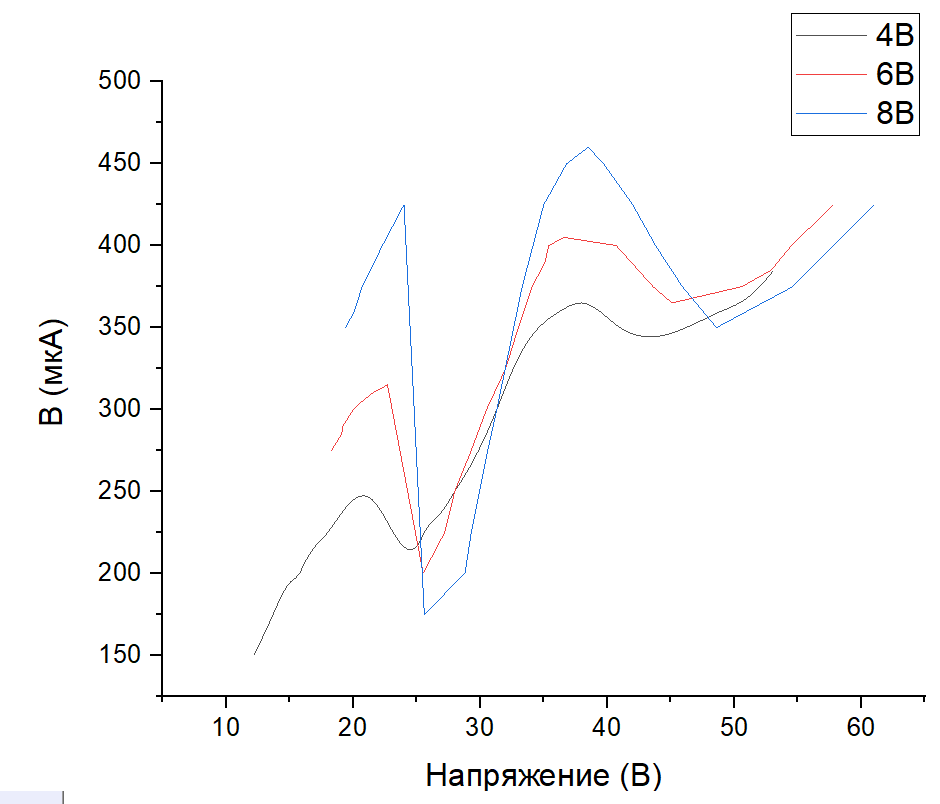
\includegraphics[scale=0.5]{1.png}
\end{figure*}
\begin{figure*}[]
	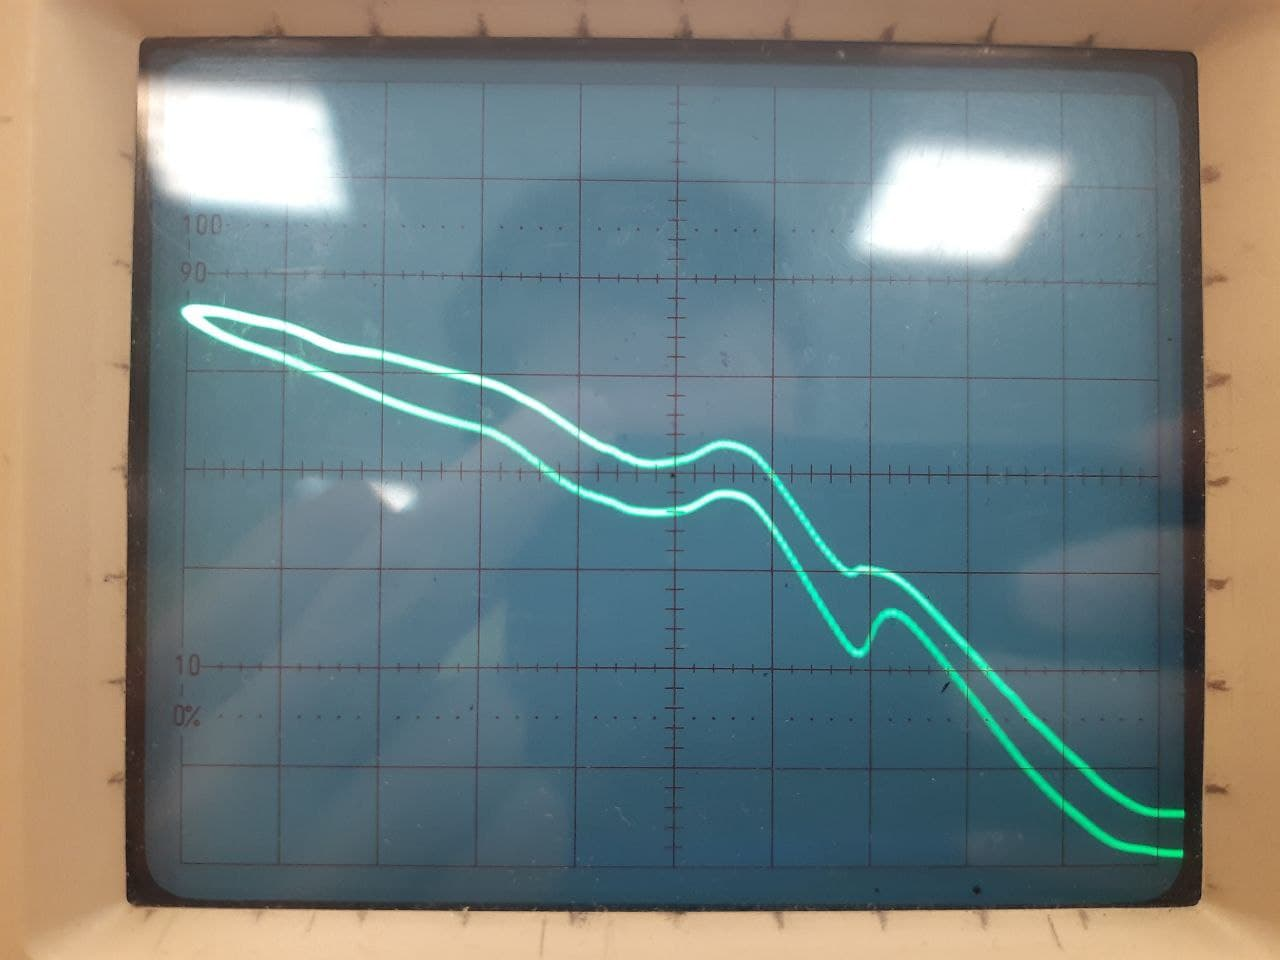
\includegraphics[scale=0.4]{2.jpg}
\end{figure*}
 
По сплайнам получается $17 \pm 1 $ эВ, по осциллографу $7 \pm 1$ эВ. Эталонное значение равно $21,2$ эВ.
\section{Заключение.}

В результате работы получены два значения для энергии возбуждения гелия, близкие к эталону.

\end{document}